%%%%%%%%%%%%%%%%%%%%%%%%%%%%%%%%%%%%%%%%%
% Beamer Presentation
% LaTeX Template
% Version 1.0 (10/11/12)
%
% This template has been downloaded from:
% http://www.LaTeXTemplates.com
%
% License:
% CC BY-NC-SA 3.0 (http://creativecommons.org/licenses/by-nc-sa/3.0/)
%
%%%%%%%%%%%%%%%%%%%%%%%%%%%%%%%%%%%%%%%%%

%----------------------------------------------------------------------------------------
%	PACKAGES AND THEMES
%----------------------------------------------------------------------------------------

\documentclass{beamer}

\mode<presentation> {

% The Beamer class comes with a number of default slide themes
% which change the colors and layouts of slides. Below this is a list
% of all the themes, uncomment each in turn to see what they look like.

%\usetheme{default}
%\usetheme{AnnArbor}
%\usetheme{Antibes}
%\usetheme{Bergen}
%\usetheme{Berkeley}
%\usetheme{Berlin}
%\usetheme{Boadilla}
\usetheme{CambridgeUS}
%\usetheme{Copenhagen}
%\usetheme{Darmstadt}
%\usetheme{Dresden}
%\usetheme{Frankfurt}
%\usetheme{Goettingen}
%\usetheme{Hannover}
%\usetheme{Ilmenau}
%\usetheme{JuanLesPins}
%\usetheme{Luebeck}
%\usetheme{Madrid}
%\usetheme{Malmoe}
%\usetheme{Marburg}
%\usetheme{Montpellier}
%\usetheme{PaloAlto}
%\usetheme{Pittsburgh}
%\usetheme{Rochester}
%\usetheme{Singapore}
%\usetheme{Szeged}
%\usetheme{Warsaw}

% As well as themes, the Beamer class has a number of color themes
% for any slide theme. Uncomment each of these in turn to see how it
% changes the colors of your current slide theme.

%\usecolortheme{albatross}
%\usecolortheme{beaver}
%\usecolortheme{beetle}
%\usecolortheme{crane}
%\usecolortheme{dolphin}
%\usecolortheme{dove}
%\usecolortheme{fly}
%\usecolortheme{lily}
%\usecolortheme{orchid}
%\usecolortheme{rose}
%\usecolortheme{seagull}
%\usecolortheme{seahorse}
%\usecolortheme{whale}
%\usecolortheme{wolverine}

%\setbeamertemplate{footline} % To remove the footer line in all slides uncomment this line
%\setbeamertemplate{footline}[page number] % To replace the footer line in all slides with a simple slide count uncomment this line

%\setbeamertemplate{navigation symbols}{} % To remove the navigation symbols from the bottom of all slides uncomment this line
}

\usepackage{graphicx} % Allows including images
\usepackage{booktabs} % Allows the use of \toprule, \midrule and \bottomrule in tables
\usepackage{multimedia}
\usepackage{hyperref}
\usepackage{subcaption}
\usepackage{multirow}
\usepackage{color}
\usepackage{wrapfig}
\usepackage{verbatim}

%----------------------------------------------------------------------------------------
%	TITLE PAGE
%----------------------------------------------------------------------------------------

\title[Convolutional Networks]{Fully Convolutional Architectures for Multi-Part Body Segmentation} % The short title appears at the bottom of every slide, the full title is only on the title page

\author{Juan Borrego Carazo} % Your name
\institute[UB] % Your institution as it will appear on the bottom of every slide, may be shorthand to save space
{
University of Barcelona \\ % Your institution for the title page
\medskip
Fundamentals of Data Science
}
\date{\today} % Date, can be changed to a custom date

\begin{document}

\begin{frame}
\titlepage % Print the title page as the first slide
\end{frame}

\begin{frame}
\frametitle{Overview} % Table of contents slide, comment this block out to remove it
\tableofcontents % Throughout your presentation, if you choose to use \section{} and \subsection{} commands, these will automatically be printed on this slide as an overview of your presentation
\end{frame}

%----------------------------------------------------------------------------------------
%	PRESENTATION SLIDES
%----------------------------------------------------------------------------------------

%------------------------------------------------
\section{Introduction} % Sections can be created in order to organize your presentation into discrete blocks, all sections and subsections are automatically printed in the table of contents as an overview of the talk
%------------------------------------------------

\begin{frame}
\huge{\centerline{\textbf{Introduction}}}
\end{frame}

%------------------------------------------------------

\begin{frame}
\frametitle{Introduction and Background}

Mechanism:

\begin{center}
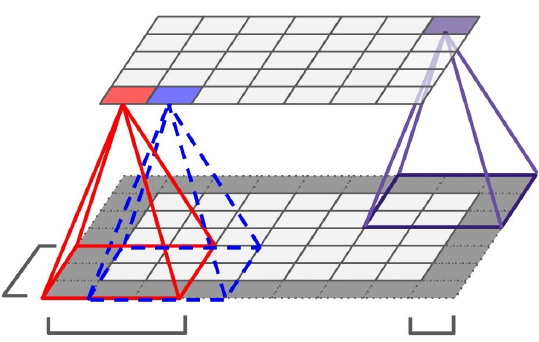
\includegraphics[scale=0.2]{convolution.png}
\end{center}

\begin{itemize}
\item Appearance of powerful baseline architecture: FCN (Fully Convolutional Network)
\item \textbf{Task}: semantic segmentation
\item Spread of use:
\begin{itemize}
\item Other tasks such as Object Detection: Mask R-CNN
\item Possibility of inclusion in other structures: Encoder-decoders
\item Modification: dilated convolutions
\item Connected to other techniques, such as CRF
\end{itemize}
\end{itemize}

\end{frame}

%----------------------------------------------------------------------------------------

\begin{frame}
\frametitle{Applications}

And the reasons behind the spread are?

\begin{itemize}
\item Reduction of parameters in networks compared to Fully Connected Networks.
\item Excellent feature extractor
\item Widespread use in applications and data types:
\begin{itemize}
\item Action recognition
\item Cancer detection
\item Aerial images
\end{itemize}
\end{itemize}


\begin{columns}
\column{.4\textwidth} 
\begin{center}
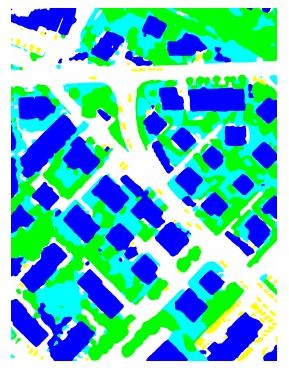
\includegraphics[scale=0.3]{aerialgt.png}
\end{center}
\column{.4\textwidth}
\begin{center}
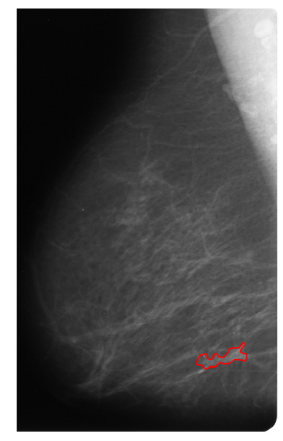
\includegraphics[scale=0.3]{mama.png}
\end{center}
\end{columns}


\end{frame}

%----------------------------------------------------------------------------------------

\begin{frame}
\frametitle{Our case $\&$ Purpose}

\textbf{Purpose}:

\begin{itemize}
\item Study the performance and behavior of architectures based fundamentally on convolutions in a specific dataset: SURREAL (Synthetic hUmans foR REal tasks)
\end{itemize}

\textbf{Work definition}: regarding the nature of our data, the work will be divided in two parts
\begin{itemize}
\item General purposed architectures
\item Human body specific architectures
\end{itemize}

\end{frame}

%-------------------------------------------------------------------------------------
\section{Dataset}
%----------------------------------------------------------------------------------------
\begin{frame}
\huge{\centerline{\textbf{Dataset}}}
\end{frame}

%-----------------------------------------------

\begin{frame}
\frametitle{Dataset}

Main characteristics:

\begin{itemize}
\item 6.5 million frames grouped into 67582 continuous image sequences of size 320x240 (RGB).
\item Synthetic human bodies displayed into a non related background.
\item Rich information attached: optical flow, body part segmentation, depth, 3D and
2D joints and surface normals.
\item \textbf{Body part ground truth segmentation}: 24 body parts each one associated with an integer index (1-24)
\end{itemize}
\begin{center}
\href{run:01_01_c0008.mp4}{
\textbf{Example}}
\end{center}
\end{frame}

%-------------------------------------------------------------------------------------

\begin{frame}
\frametitle{Dataset Modifications}

Process to obtain final dataset:

\begin{itemize}
\item Cut frames and relate them to corresponding GT matrix.
\item Crop images with the body on the center.
\item Correct GT with parts mislabeled.
\item With K-means algorithm create train, validation and test set base on 3D joints information.
\item Train: 90k images, Validation: 15k and Test 15k images
\end{itemize}

\end{frame}

%--------------------------------------------------------------

\begin{frame}
\frametitle{Dataset example}

\begin{figure}
\centering
\begin{subfigure}{.3\textwidth}
  \centering
  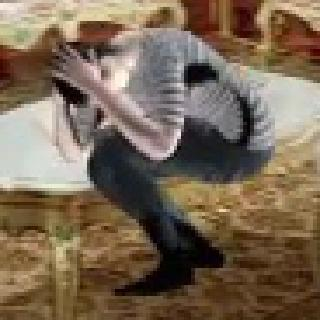
\includegraphics[scale=0.25]{ung_77_09_c0001_67.jpg}
\end{subfigure}
\begin{subfigure}{.3\textwidth}
  \centering
  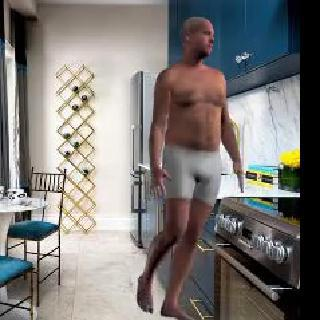
\includegraphics[scale=0.25]{ung_91_62_c0003_87.jpg}
\end{subfigure}
\begin{subfigure}{.3\textwidth}
  \centering
  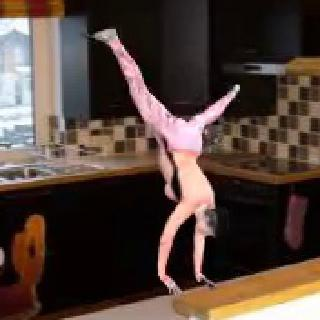
\includegraphics[scale=0.25]{ung_144_02_c0006_2.jpg}
\end{subfigure}\\
\begin{subfigure}{.3\textwidth}
  \centering
  
\includegraphics[scale=0.25]{ung_77_09_c0001_segm_67.png}
\end{subfigure}
\begin{subfigure}{.3\textwidth}
  \centering
  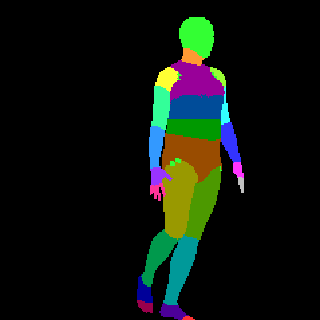
\includegraphics[scale=0.25]{ung_91_62_c0003_segm_87.png}
\end{subfigure}
\begin{subfigure}{.3\textwidth}
  \centering
  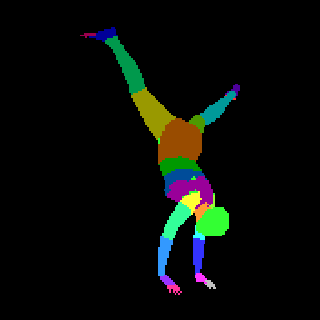
\includegraphics[scale=0.25]{ung_144_02_c0006_segm_2.png}
\end{subfigure}

\caption{First row: sample images. Second row: corresponding ground truths}
\label{dataset:samples}
\end{figure}

\end{frame}

%-------------------------------------------------------------------------------------
\section{Network study}
%----------------------------------------------------------------------------------------
\begin{frame}
\huge{\centerline{\textbf{General purposed networks}}}
\end{frame}

%-----------------------------------------------

\begin{frame}
\frametitle{Experimental Procedure}

Take the baseline network and:

\begin{itemize}
\item Doubling the convolutional filters
\item Data augmentation: mirroring and scaling.
\item Class balancing through loss weighting
\end{itemize}

Class balancing strategy 

\begin{itemize}
\item \textbf{Direct} $L = -\sum_{i}y_{i}\log{softmax(x_{i}w_{i})}$
\item \textbf{Outter} $L = -\sum_{i}w_{i}y_{i}\log{softmax(w_{i})}$
\end{itemize}

 
and weights (C is the number of pixels of each class)

\begin{itemize}
\item \textbf{Inverse Frequency}: $W_{i} = 1 -\frac{C_{i}}{\sum_{i}C_{i}}$
\item \textbf{Exponential weights}: \begin{eqnarray*}
B = \frac{max(C)}{C}\\
W = B e^{-\frac{1}{4}\frac{B-mean(B)}{std{B}}} 
\end{eqnarray*}
\end{itemize}

\end{frame}
%-------------------------------------------------------------------------------------

\subsection{ICNet}

\begin{frame}
\huge{\centerline{\textbf{ICNet}}}
\end{frame}

%-----------------------------------------------

\begin{frame}
\frametitle{Network Description}

\begin{columns}
\column{.3\textwidth} 
\textbf{General architecture}\\
\begin{equation*}
L = \lambda_{1}L_{1} + \lambda_{2}L_{2} + \lambda_{3}L_{3}
\end{equation*}

\column{.65\textwidth}
\begin{center}
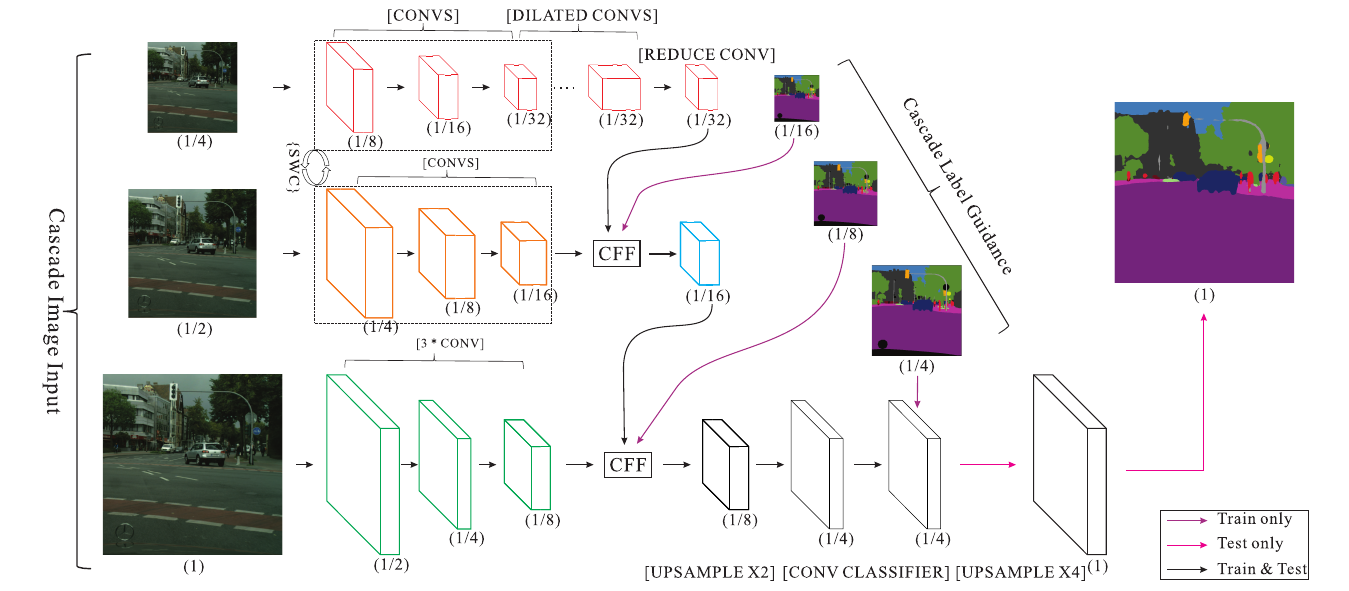
\includegraphics[scale=0.2]{icnet.png}
\end{center}
\end{columns}
\begin{columns}
\column{.3\textwidth}

\textbf{Cascade Feature Fusion}
\flushleft{\tiny{ICNet for Real-Time Semantic Segmentation on High-Resolution Images. \textit{Zhao H. et al.}, \href{url}{https://arxiv.org/abs/1704.08545}}}
\column{.65\textwidth}
\begin{center}
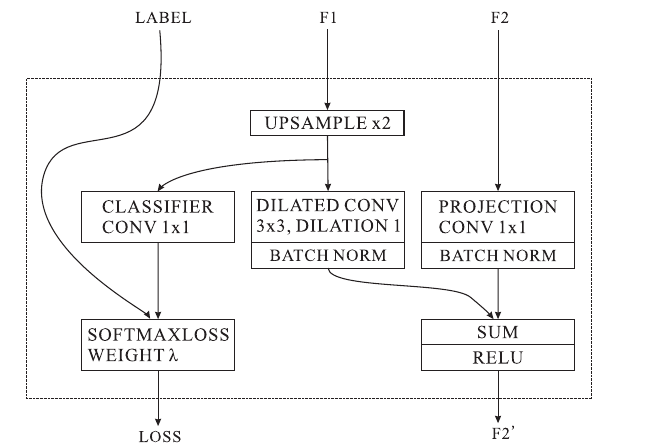
\includegraphics[scale=0.3]{ccf.png}
\end{center}
\end{columns}

\end{frame}
%-------------------------------------------------------------------------------------

\begin{frame}
\frametitle{Results and Analysis}

\begin{table}[h!]
  \begin{center}
    \resizebox{.7\textwidth}{!}{
    \begin{tabular}{|c|c|c|c|} % <-- Changed to S here.
      \textbf{Architecture} & \textbf{mIoU ($\%$)} & \textbf{Accuracy ($\%$)} & \textbf{F1 ($\%$)} \\
      \hline
      Normal & 38.19 & 94.64 & 88.17\\
      \hline
      Doubled filters & 27.51 & 93.01 & 84.97\\  
      \hline
      Normal + Data Aug. & 32.60 & 91.15 & 91.61\\
    \end{tabular}}
    \caption{Results for the different ablation results in the validation set.}
    \label{icnet:table1}
  \end{center}
\end{table}

\small{Notice batch normalization inclusion into training.}
\begin{columns}
\column{.4\textwidth} 
\begin{center}
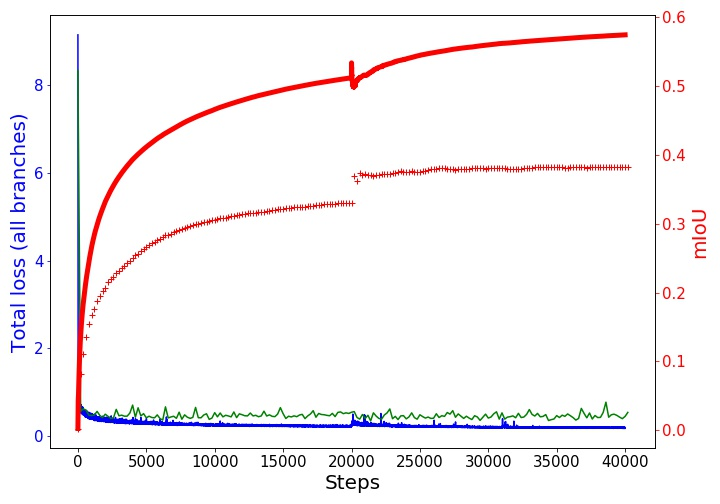
\includegraphics[scale=0.2]{icnet_res_1.jpg}
\end{center}
\column{.4\textwidth}
\begin{center}
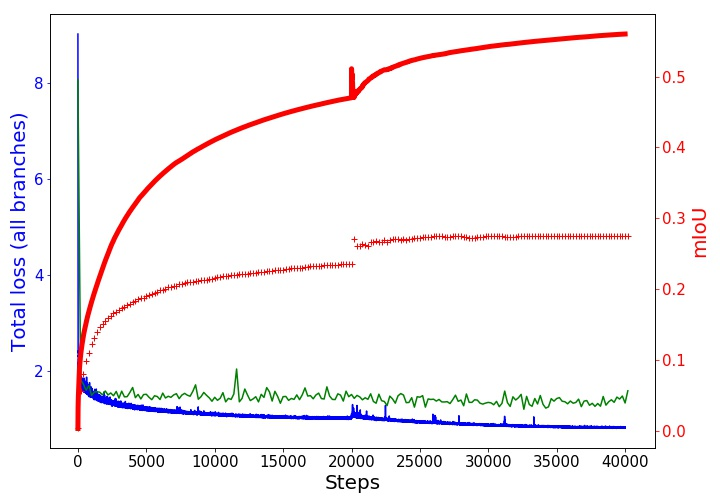
\includegraphics[scale=0.2]{icnet_res_2.jpg}
\end{center}
\end{columns}

\end{frame}
%-------------------------------------------------------------------------------------

\begin{frame}
\frametitle{Class balancing results}

\begin{table}[h!]
  \begin{center}
    \resizebox{\textwidth}{!}{
    \begin{tabular}{|c|c|c|c|c|c|c|c|c|c|c|c|c|c|c|c|c|c|c|c|c|c|} % <-- Changed to S here.
    &\textbf{mIoU ($\%$)}&\multicolumn{14}{c|}{\textbf{Accuracy per Class}($\%$)}\\
    \hline
      \textbf{Architecture} & \textbf{All Classes} & \textbf{All Classes}& \textbf{Background} & \textbf{Head} & \textbf{Torso} & \textbf{U.Legs}& \textbf{L.Legs} & \textbf{Neck} & \textbf{Shoulder} & \textbf{U.Arms}& \textbf{L.Arms}& \textbf{Feets}& \textbf{Hands}& \textbf{Fingers} & \textbf{Toes}  \\
      \hline
      Normal & \textcolor{red}{38.2} & 48.7 & 98.9 & 84.9 & 74.78 & 64.3 & 53.8 & 64.0 & 54.2 & 52.7 & 39.5 & 32.3 & 19.8 & \textcolor{red}{9.3} & \textcolor{red}{9.5} \\
 	  \hline
      W1 (Outer) & 37.5 & 52.3 & 97.7 & 90.0  & 74.8 & 70.9 & 61.7 & 60.9 & 56.0 & 57.34 & 50.1 & 38.9 & 22.9 & 10.2 &  11.3\\  
      \hline
      W1 (Direct) & 6.5 & 7.9& 99.9 & 6.13 & 15.5 & 7.7 & 0.8 & 0.0  & 4.7 & 1.9 & 0.0 &3.6 & 0.0 & 0.0 & 0.0\\
      \hline
      W2 (Outer) & 25.8 & \textcolor{red}{54.8} & 89.2 & 89.3 & 61.6 & 64.1 & 65.2 & 72.4 & 60.3 & 47.0 & 46.03 & 52.35 & 33.4& \textcolor{red}{31.0} & \textcolor{red}{36.9} \\
      \hline
      W2 (Direct) & 25.5 & 34.0 & 99.3 & 78.7 & 70.7 & 70.0 & 59.0 & 1.9 & 8.9 & 32.9 & 15.7 & 7.1 & 0.5 & 0.0 & 0 .0 \\
    \end{tabular}}
    \caption{Performance results on validation dataset for the original structure and the architecture with loss weighting for each setup. Here W1 indicates the inverse frequency weithing and W2 the exponential weighting. Best values enclosed in [].}
    \label{icnet:table2}
  \end{center}
\end{table}

\end{frame}
%-------------------------------------------------------------------------------------


\begin{frame}
\frametitle{Final and Qualitative Results}

\begin{table}[h!]
  \begin{center}
    \resizebox{.6\textwidth}{!}{
    \begin{tabular}{|c|c|c|c|} % <-- Changed to S here.
      \textbf{Architecture} & \textbf{mIoU ($\%$)} & \textbf{Accuracy ($\%$)} & \textbf{F1 ($\%$)} \\
      \hline
      Normal & 45.14 & 95.76 & 89.73\\
    \end{tabular}}
    
    \label{icnet:table3}
  \end{center}
\end{table}


\begin{figure}
\centering
\begin{subfigure}{.3\textwidth}
\centering
  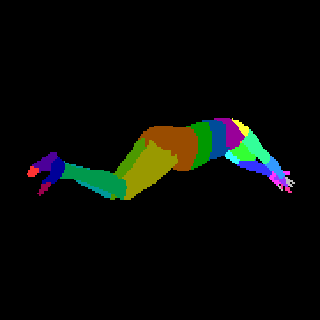
\includegraphics[scale=0.21]{ung_126_09_c0008_segm_85_gt.png}
\end{subfigure}
\begin{subfigure}{.3\textwidth}
  \centering
  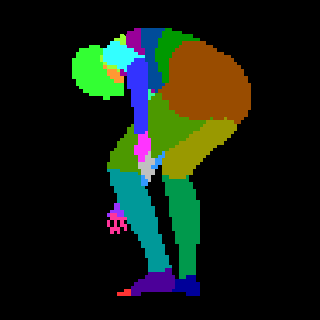
\includegraphics[scale=0.21]{ung_137_31_c0008_segm_77_gt.png}
\end{subfigure}
\begin{subfigure}{.3\textwidth}
  \centering
  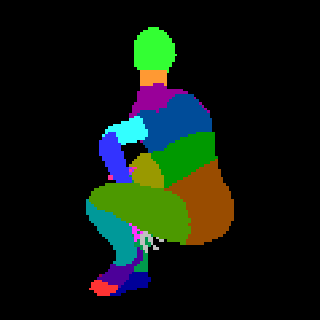
\includegraphics[scale=0.21]{19_12_c0006_segm_29_gt.png}
\end{subfigure}
\end{figure}
\begin{figure}
\centering
\begin{subfigure}{.31\textwidth}
\centering
  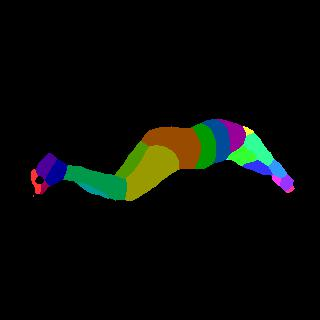
\includegraphics[scale=0.21]{ung_126_09_c0008_85.jpg}
\end{subfigure}%
\begin{subfigure}{.3\textwidth}
  \centering
  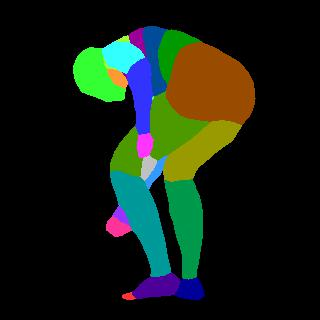
\includegraphics[scale=0.21]{ung_137_31_c0008_77.jpg}
\end{subfigure}
\begin{subfigure}{.3\textwidth}
  \centering
  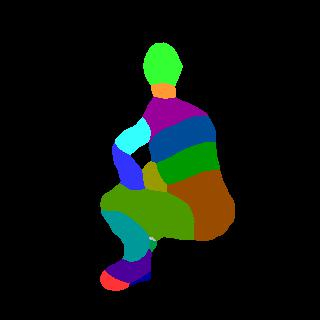
\includegraphics[scale=0.21]{19_12_c0006_29.jpg}
\end{subfigure}
\end{figure}



\end{frame}

%-------------------------------------------------------------------------------------

\subsection{SegNet}

\begin{frame}
\huge{\centerline{\textbf{SegNet}}}
\end{frame}

%-----------------------------------------------

\begin{frame}
\frametitle{Network Description}

\begin{columns}
\column{.3\textwidth} 
\textbf{General architecture}\\


\column{.65\textwidth}
\begin{center}
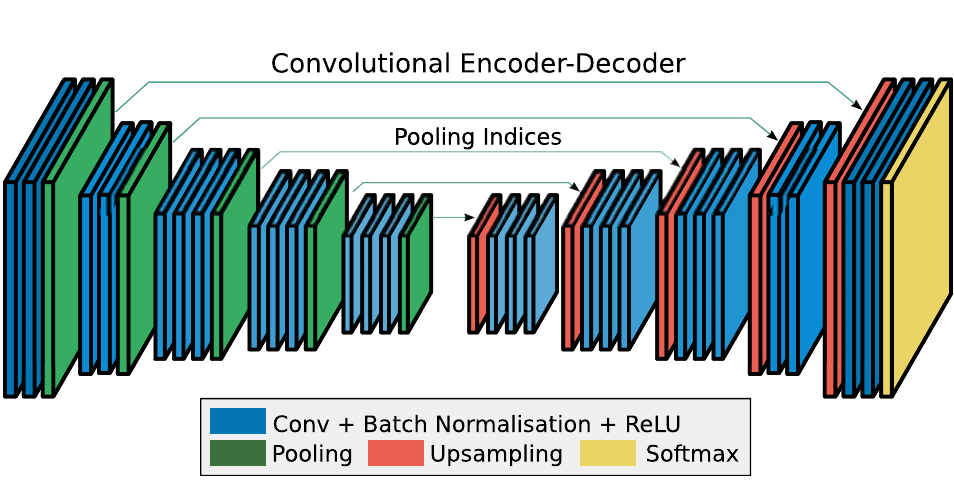
\includegraphics[scale=0.3]{seg_net.png}
\end{center}
\end{columns}
\begin{columns}
\column{.4\textwidth}

\textbf{Index Skip connections}
\flushleft{\tiny{ SegNet: A Deep Convolutional Encoder-Decoder Architecture for Robust Semantic Pixel-Wise Labelling. \textit{Badrinarayanan, V.},\href{url}{https://arxiv.org/abs/1505.07293}}}
\column{.55\textwidth}
\begin{center}
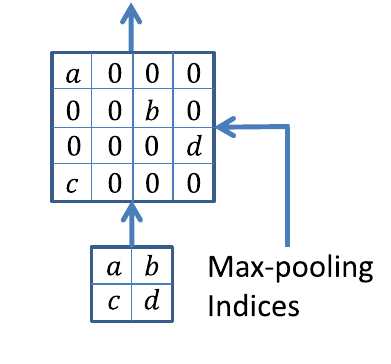
\includegraphics[scale=0.3]{seg_idx.png}
\end{center}
\end{columns}

\end{frame}
%-------------------------------------------------------------------------------------

\begin{frame}
\frametitle{Results and Analysis}

\begin{table}[h!]
  \begin{center}
    
    \begin{tabular}{|c|c|c|c|} % <-- Changed to S here.
      \textbf{Architecture} & \textbf{mIoU ($\%$)} & \textbf{Accuracy ($\%$)} & \textbf{F1 ($\%$)} \\
      \hline
      Normal & 38.80 & 94.87 & 54.34\\
      \hline
      Doubled filters & 39.17 & 94.79  & 54.49 \\  
      \hline
      Doubled Filters + Data Aug. & 23.28 & 89.24 & 33.21\\
    \end{tabular}

    \label{segnet:table1}
  \end{center}
\end{table}

\begin{columns}
\column{.4\textwidth} 
\begin{center}
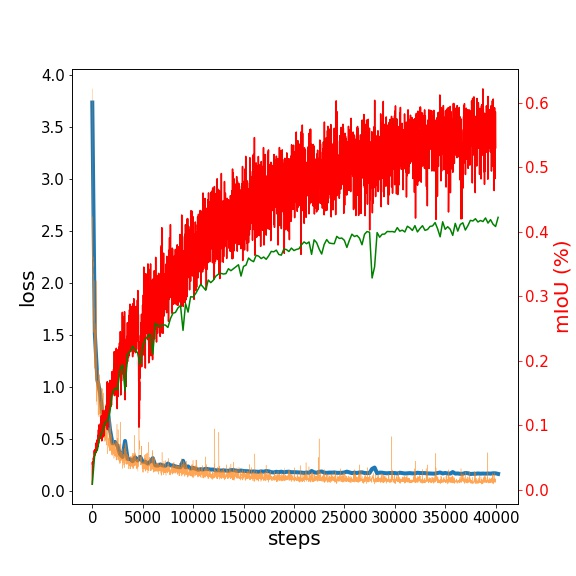
\includegraphics[scale=0.22]{seg_res_1.jpg}
\end{center}
\column{.4\textwidth}
\begin{center}
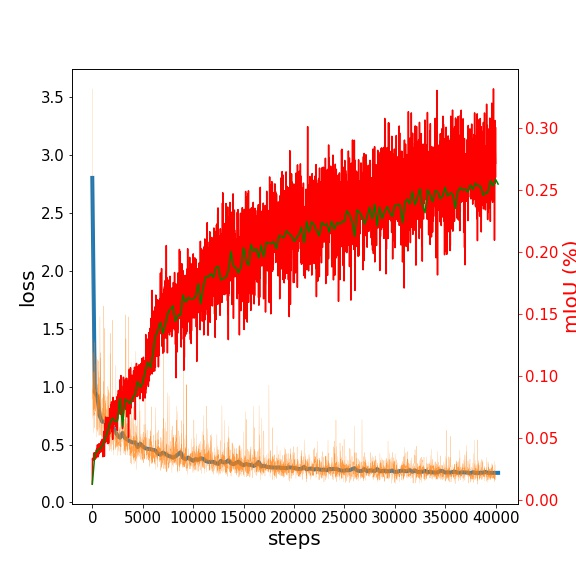
\includegraphics[scale=0.22]{seg_res_2.jpg}
\end{center}
\end{columns}

\end{frame}
%-------------------------------------------------------------------------------------

\begin{frame}
\frametitle{Class balancing results}

\begin{table}[h!]
  \begin{center}
    \resizebox{\textwidth}{!}{
    \begin{tabular}{|c|c|c|c|c|c|c|c|c|c|c|c|c|c|c|c|c|c|c|c|c|c|c|} % <-- Changed to S here.
    &\textbf{mIoU ($\%$)}&\multicolumn{12}{c}{\textbf{Accuracy per Class}($\%$)}\\
    \hline
      \textbf{Architecture} & \textbf{All Classes} & \textbf{All classes}&\textbf{Background} & \textbf{Head} & \textbf{Torso} & \textbf{U.Legs}& \textbf{L.Legs} & \textbf{Neck} & \textbf{Shoulder} & \textbf{U.Arms}& \textbf{L.Arms}& \textbf{Feets}& \textbf{Hands}& \textbf{Fingers} & \textbf{Toes}  \\
      \hline
      Double Filters & \textcolor{red}{39.17}  & 49.9 & 99.1 & 84.2 & 70.9 & 63.2 & 58.4 & 58.1 & 51.8 & 52.7 & 43.9 & 39.9 & 28.8 & 12.4 & 9.8 \\
 	  \hline
      DF + W1 (Outer) & 38.8 & 55.6 & 97.5 & 90.3 & 74.2 & 66.8 & 61.8 & 58.3 & 65.1 & 62.0 & 49.6 & 42.0 & 36.3 & 25.3 &  14.2\\  
      \hline
      DF + W2 (Outer) & 21.65 & \textcolor{red}{56.3} & 78.18 & 79.8 & 65.6 & 60.0 & 57.1 & 85.8 & 71.1 & 52.5 & 51.8 & 44.2 & 41.7 & 34.1 & 38.4 \\

    \end{tabular}}
    \caption{Performance results on validation dataset for the doubled filter structure and the same architecture but with loss weighting for each setup. Here W1 indicates the inverse frequency weithing and W2 the exponential weighting (DF, i.e. doubled filters). Between brackets the best perfoming scheme in both mIoU and mean Accuracy per class.}
    \label{segnet:table2}
  \end{center}
\end{table}


\end{frame}
%-------------------------------------------------------------------------------------


\begin{frame}
\frametitle{Final and Qualitative Results}

\begin{table}[h!]
  \begin{center}
    
    \begin{tabular}{|c|c|c|c|} % <-- Changed to S here.
      \textbf{Architecture} & \textbf{mIoU ($\%$)} & \textbf{Accuracy ($\%$)} & \textbf{F1 ($\%$)} \\
      \hline
      Normal & 33.59 & 94.62 & 44.32\\
    \end{tabular}
   
    \label{segnet:table3}
  \end{center}
\end{table}

\begin{figure}
\centering
\begin{subfigure}{.3\textwidth}
\centering
  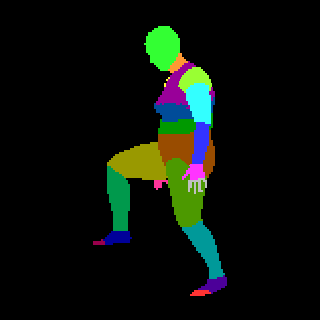
\includegraphics[scale=0.21]{36_04_c0001_segm_30.png}
\end{subfigure}
\begin{subfigure}{.3\textwidth}
  \centering
  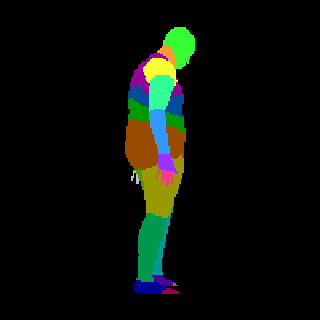
\includegraphics[scale=0.21]{36_16_c0002_segm_34.png}
\end{subfigure}
\begin{subfigure}{.3\textwidth}
  \centering
  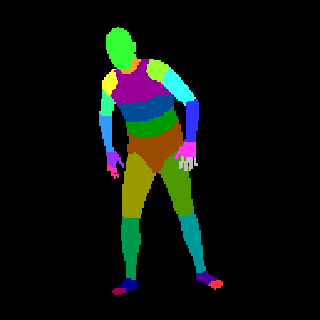
\includegraphics[scale=0.21]{104_52_c0002_segm_38.png}
\end{subfigure}

\end{figure}
\begin{figure}
\begin{subfigure}{.3\textwidth}
\centering
  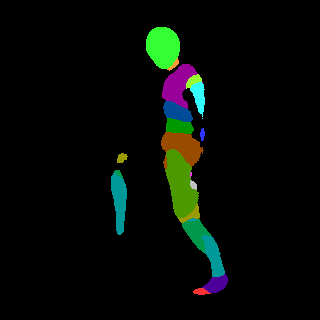
\includegraphics[scale=0.21]{36_04_c0001_segm_30_seg.png}
\end{subfigure}%
\begin{subfigure}{.3\textwidth}
  \centering
  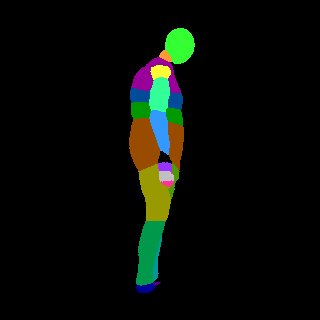
\includegraphics[scale=0.21]{36_16_c0002_segm_34_seg.png}
\end{subfigure}
\begin{subfigure}{.3\textwidth}
  \centering
  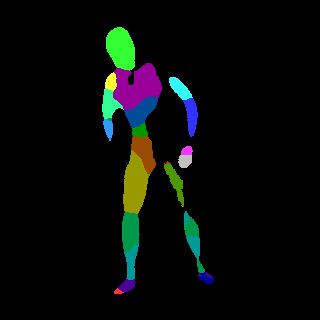
\includegraphics[scale=0.21]{104_52_c0002_segm_38_seg.png}
\end{subfigure}

\label{segnet:inference}
\end{figure}


\end{frame}

%-----------------------------------------------------------------------------------
\begin{frame}
\huge{\centerline{\textbf{Specific Purpose Network:}}}
\huge{\centerline{\textbf{Stacked Hourglass}}}
\end{frame}
%-------------------------------------------------------------------------------------

\subsection{Stacked Hourglass Network}




%--------------------------------------------------------------------------------

\begin{frame}
\frametitle{Network Description}

\begin{itemize}
\item Originally intended to human pose estimation
\item Same bottom-up top-down structure stacked several times
\item Allows for refinement of the output produced.
\end{itemize}
\begin{center}
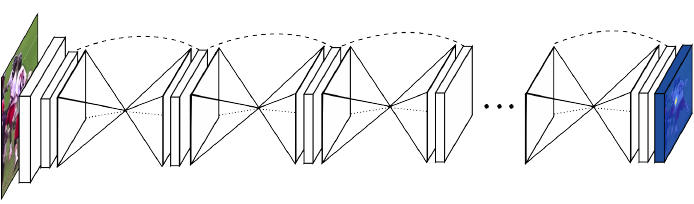
\includegraphics[scale=0.5]{stacked.png}
\end{center}
\flushleft{\tiny{ Stacked Hourglass Networks for Human Pose Estimation. \textit{Newell, A.},\href{url}{https://arxiv.org/abs/1603.06937}}}

\end{frame}
%-------------------------------------------------------------------------------------

%--------------------------------------------------------------------------------

\begin{frame}
\frametitle{Network Description}

\begin{columns}
\column{.3\textwidth} 
\textbf{Hourglass Module}\\


\column{.65\textwidth}
\begin{center}
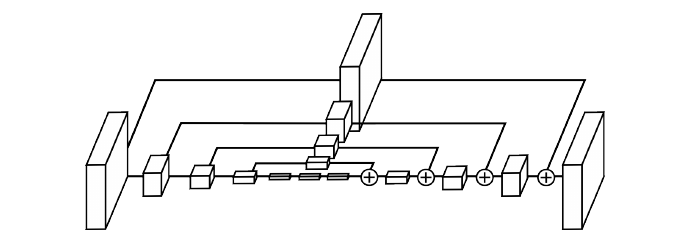
\includegraphics[scale=0.4]{hourmodule.png}
\end{center}
\end{columns}
\begin{columns}
\column{.3\textwidth}

\textbf{Residual module $\&$ Intermediate Supervision }
\column{.65\textwidth}
\begin{center}
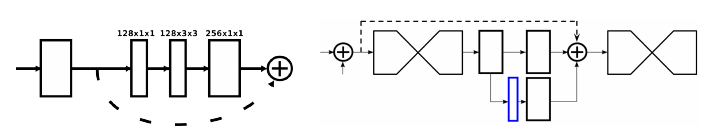
\includegraphics[scale=0.4]{residual.png}
\end{center}
\end{columns}

\end{frame}
%-------------------------------------------------------------------------------------

\begin{frame}
\frametitle{Experimental Procedure}

\begin{itemize}
\item Two experiments:
\begin{itemize}
\item Different GT resolutions for each intermediate supervision step (i.e. for each hourglass module)
\item A multi-task branch is added to the main pipeline: Joint position determination.
\end{itemize}
\end{itemize}
\begin{figure}
\centering
\begin{subfigure}{.19\textwidth}
\centering
  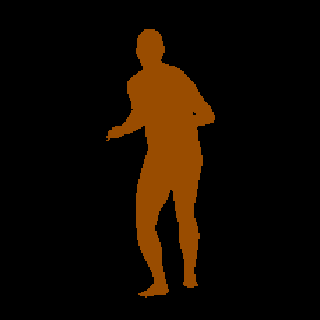
\includegraphics[scale=0.3]{02_05_c0005_segm_80_2c.png}
\end{subfigure}
\begin{subfigure}{.19\textwidth}
  \centering
  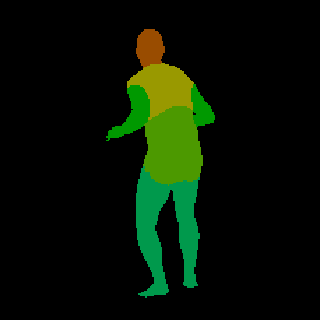
\includegraphics[scale=0.3]{02_05_c0005_segm_80_6c.png}
\end{subfigure}
\begin{subfigure}{.19\textwidth}
  \centering
  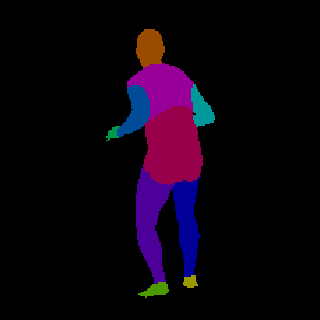
\includegraphics[scale=0.3]{02_05_c0005_segm_80_12c.png}
\end{subfigure}
\begin{subfigure}{.19\textwidth}
  \centering
  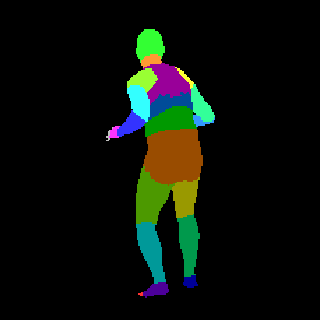
\includegraphics[scale=0.3]{02_05_c0005_segm_80_25c.png}\\
\end{subfigure}\\
\caption{\textbf{1st Experiment}, different ground truth resolutions, one for each module. The idea is to learn a progressive refinement of the real ground truth.}
\label{hourglass:diffgrounds}
\end{figure}


\end{frame}
%-------------------------------------------------------------------------------------

\begin{frame}
\frametitle{Network Description}

\begin{columns}
\column{.45\textwidth} 
\begin{center}
\textbf{Multi-task branch}\\


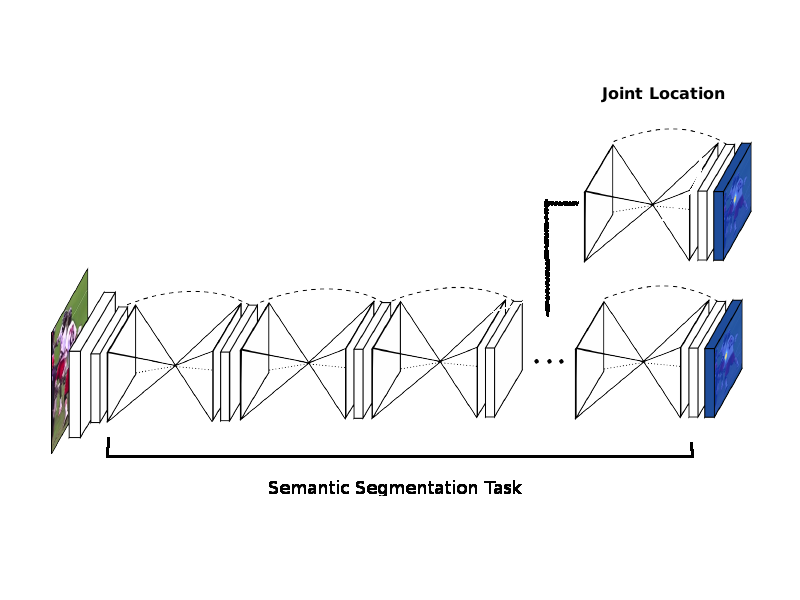
\includegraphics[scale=0.2]{multitask.png}
\end{center}

\column{.45\textwidth}
\begin{center}
\textbf{Human body joints}

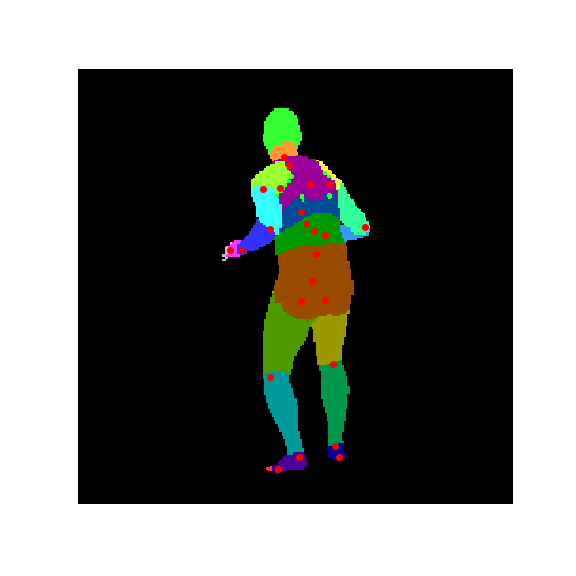
\includegraphics[scale=0.23]{surreal_joints.png}
\end{center}
\end{columns}

\end{frame}
%-------------------------------------------------------------------------------------
\begin{frame}
\frametitle{Results and Analysis}

\begin{table}[h!]
  \begin{center}
    
    \begin{tabular}{|c|c|c|c|} % <-- Changed to S here.
      \textbf{Architecture} & \textbf{mIoU ($\%$)} & \textbf{Accuracy ($\%$)} & \textbf{F1 ($\%$)} \\
      \hline
      Original & 63.19 & 98.75 & 95.24\\
      \hline
      O. + GT resolutions & 16.22 & 90.58 & 61.98\\  
      \hline
      O. + Multitask Head & 58.05 & 97.18 & 96.05\\
    \end{tabular}
    
    \label{hourglass:table1}
  \end{center}
\end{table}

 
\begin{center}
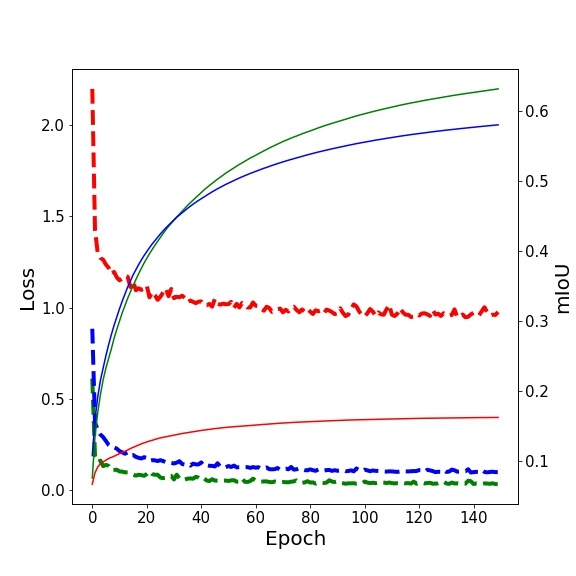
\includegraphics[scale=0.25]{loss_plot_GTnormal.jpg}
\end{center}


\end{frame}

%------------------------------------------------------------
\begin{frame}
\frametitle{Final and qualitative results}

\begin{table}[h!]
  \begin{center}
    \resizebox{!}{0.035\textwidth}{
    \begin{tabular}{|c|c|c|c|} % <-- Changed to S here.
      \textbf{Architecture} & \textbf{mIoU ($\%$)} & \textbf{Accuracy ($\%$)} & \textbf{F1 ($\%$)} \\
      \hline
      Original & 55.32 & 97.02 & 93.07\\
      \hline
    \end{tabular}}
    
  \end{center}
\end{table}
\begin{figure}
\centering
\begin{subfigure}{.3\textwidth}
\centering
  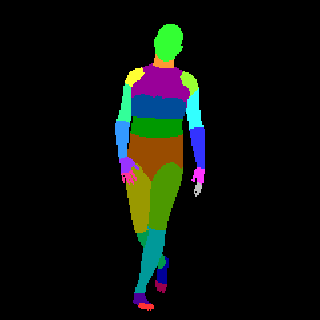
\includegraphics[scale=0.2]{ung_104_36_c0011_segm_7.png}
\end{subfigure}
\begin{subfigure}{.3\textwidth}
  \centering
  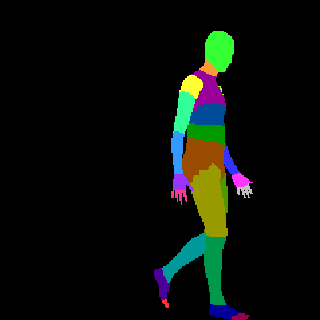
\includegraphics[scale=0.2]{40_02_c0011_segm_19.png}
\end{subfigure}
\begin{subfigure}{.3\textwidth}
  \centering
  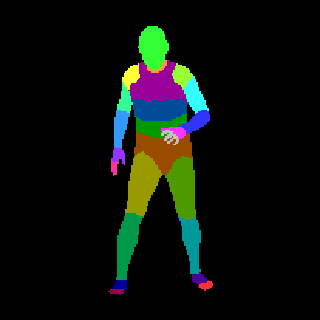
\includegraphics[scale=0.2]{104_52_c0002_segm_64.png}
\end{subfigure}
\end{figure}

\begin{figure}
\centering
\begin{subfigure}{.32\textwidth}
\centering
  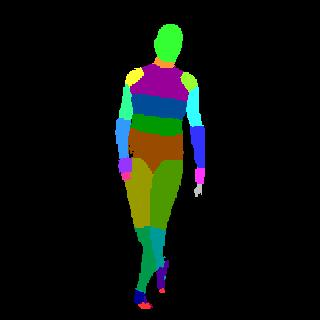
\includegraphics[scale=0.2]{ung_104_36_c0011_7.jpg}
\end{subfigure}
\begin{subfigure}{.32\textwidth}
  \centering
  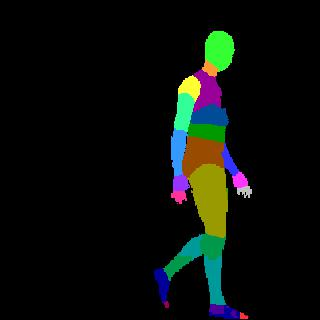
\includegraphics[scale=0.2]{40_02_c0011_19.jpg}
\end{subfigure}
\begin{subfigure}{.32\textwidth}
  \centering
  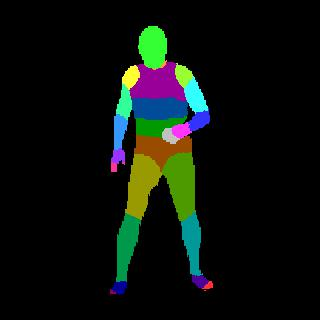
\includegraphics[scale=0.2]{104_52_c0002_64.jpg}
\end{subfigure}

\label{hourglass:inference}
\end{figure}
\end{frame}
%-------------------------------------------------------------------------------------

%-----------------------------------------------------------------------------------
\begin{frame}
\huge{\centerline{\textbf{Network Comparison}}}
\end{frame}
%-------------------------------------------------------------------------------------
\subsection{Network Comparison}

\begin{frame}
\frametitle{Test and qualitative results}

\begin{table}[h!]
  \begin{center}
    \resizebox{0.7\textwidth}{!}{
    \begin{tabular}{|c|c|c|c|} % <-- Changed to S here.
      \textbf{Architecture} & \textbf{mIoU ($\%$)} & \textbf{Accuracy ($\%$)} & \textbf{F1 ($\%$)} \\
      \hline
      ICNet & 45.14 & 95.76 & 89.73\\
      \hline
      SegNet & 33.59 & 94.62  & 44.32 \\  
      \hline
      Stacked Hourglass & 55.32 & 97.02 & 93.07\\
    \end{tabular}}
    \label{final:table1}
  \end{center}
\end{table}

\begin{itemize}
\item Differences between networks:
\begin{itemize}
\item \textbf{ICNet}, 3 branches different resolutions. Only upper branch used in testing. 6,743,733 trainable variables.
\item \textbf{SegNet}, encoder-decoder with skip connections. 5,904,921 trainable variables.
\item \textbf{Stacked Hourglass}: concatenated downsampling-upsampling with residual modules. 14,804,962 trainable variables.
\end{itemize}
\item Raises the following question: which is the reasons behind the difference in performance:
\begin{itemize}
\item Size of network?
\item Suitability to data type?
\end{itemize}
\end{itemize}

\end{frame}

%-----------------------------------------------
\begin{frame}
\frametitle{Qualitative Results}

\begin{figure}
GT
\centering
\begin{subfigure}{.19\textwidth}
\centering
  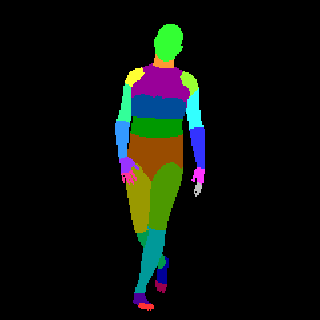
\includegraphics[scale=0.12]{ung_104_36_c0011_segm_7.png}
\end{subfigure}
\begin{subfigure}{.19\textwidth}
  \centering
  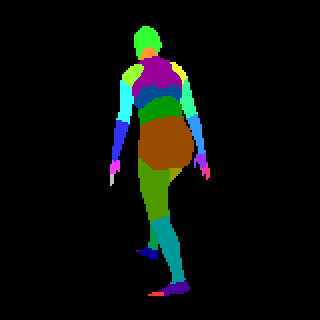
\includegraphics[scale=0.12]{36_10_c0019_segm_10.png}
\end{subfigure}
\begin{subfigure}{.19\textwidth}
  \centering
  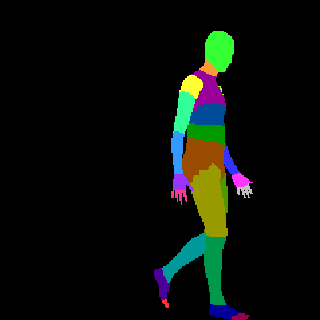
\includegraphics[scale=0.12]{40_02_c0011_segm_19.png}
\end{subfigure}
\begin{subfigure}{.19\textwidth}
  \centering
  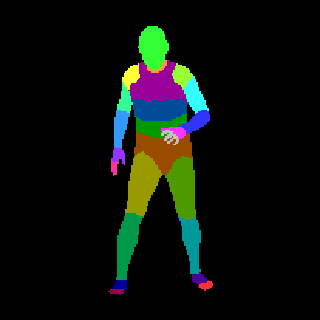
\includegraphics[scale=0.12]{104_52_c0002_segm_64.png}\\
\end{subfigure}\\
\end{figure}
\begin{figure}
ICNet
\centering
\begin{subfigure}{.198\textwidth}
\centering
  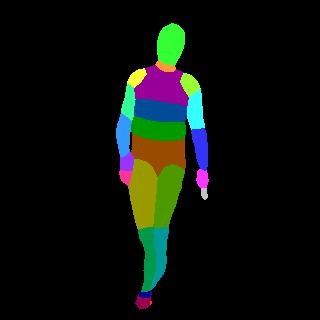
\includegraphics[scale=0.12]{ung_104_36_c0011_7_ice.jpg}
\end{subfigure}%
\begin{subfigure}{.19\textwidth}
  \centering
  \includegraphics[scale=0.12]{36_10_c0019_10_ice.jpg}
\end{subfigure}
\begin{subfigure}{.19\textwidth}
  \centering
  \includegraphics[scale=0.12]{40_02_c0011_19_ice.jpg}
\end{subfigure}
\begin{subfigure}{.189\textwidth}
  \centering
  \includegraphics[scale=0.12]{104_52_c0002_64_ice.jpg}
\end{subfigure}\\

\end{figure}
\begin{figure}
SegNet
\centering
\begin{subfigure}{.19\textwidth}
\centering
  \includegraphics[scale=0.12]{ung_104_36_c0011_segm_7_seg.png}
\end{subfigure}
\begin{subfigure}{.19\textwidth}
  \centering
  \includegraphics[scale=0.12]{36_10_c0019_segm_10_seg.png}
\end{subfigure}
\begin{subfigure}{.19\textwidth}
  \centering
  \includegraphics[scale=0.12]{40_02_c0011_segm_19_seg.png}
\end{subfigure}
\begin{subfigure}{.19\textwidth}
  \centering
  \includegraphics[scale=0.12]{104_52_c0002_segm_64_seg.png}\\
\end{subfigure}\\
\end{figure}
\begin{figure}
Hourglass
\centering
\begin{subfigure}{.198\textwidth}
\centering
  \includegraphics[scale=0.12]{ung_104_36_c0011_7.jpg}
\end{subfigure}%
\begin{subfigure}{.19\textwidth}
  \centering
  \includegraphics[scale=0.12]{36_10_c0019_10.jpg}
\end{subfigure}
\begin{subfigure}{.19\textwidth}
  \centering
  \includegraphics[scale=0.12]{40_02_c0011_19.jpg}
\end{subfigure}
\begin{subfigure}{.189\textwidth}
  \centering
  \includegraphics[scale=0.12]{104_52_c0002_64.jpg}
\end{subfigure}


\label{final:inference}
\end{figure}
\end{frame}
%-------------------------------------------------------

\begin{frame}
\huge{\centerline{\textbf{Conclusions}}}
\end{frame}
%-------------------------------------------------------------------------------------
\section{Conclusions}

\begin{frame}
\frametitle{Conclusions and future work}

\textbf{Conclusions}
\begin{itemize}
\item Three CNN analyzed: two general purposed and one data suited network. Acquired level of Tensorflow to modify adapt state of the art code.
\item Almost all ablation experiments and modifications did not overperformed original networks.
\item Main drawback of study: is it size or network specialization that drives performance?
\end{itemize}
\textbf{Future work}
\begin{itemize}
\item Include more networks
\item Adapt network parameters or size to make them comparable.
\end{itemize}
\end{frame}

%-----------------------------------------------------------------------


%------------------------------------------------

\begin{frame}
\Huge{\centerline{The End}}
\end{frame}

%-----------------------------------------------------


%-----------------------------------------------

\end{document} 
